\documentclass[aspectratio=43,english]{beamer} %If you want to create Polish presentation, replace 'english' with 'polish' and uncomment 3-th line, i.e., '\usepackage{polski}'
\usepackage[utf8]{inputenc}
\usepackage{polski} %Uncomment for Polish language
\usepackage{babel}
\usepackage{listings} %We want to put listings

\mode<beamer>{ 	%in 'beamer' mode
	\hypersetup{pdfpagemode=FullScreen}		%Enable Full screen mode
	\usetheme{JuanLesPins} 		%Show part title in right footer
	%\usetheme[dark]{AGH}                 		%Use dark background
	%\usetheme[dark,parttitle=leftfooter]{AGH}  	%Use dark background and show part title in left footer
}
\mode<handout>{	%in 'handout' mode
	\hypersetup{pdfpagemode=None}		
	\usepackage{pgfpages}
  	\pgfpagesuselayout{4 on 1}[a4paper,border shrink=5mm,landscape]	%show 4 slides on 1 page
  	\usetheme{boxes}
  	\addheadbox{structure}{\quad\insertpart\hfill\insertsection\hfill\insertsubsection\qquad} 	%content of header
 	\addfootbox{structure}{\quad\insertauthor\hfill\insertframenumber\hfill\insertsubtitle\qquad} 	%content of footer
}

\AtBeginPart{ %At begin part: display its name
	\frame{\partpage}
} 


%%%%%%%%%%% Configuration of the listings package %%%%%%%%%%%%%%%%%%%%%%%%%%
% Source: https://en.wikibooks.org/wiki/LaTeX/Source_Code_Listings#Using_the_listings_package
%%%%%%%%%%%%%%%%%%%%%%%%%%%%%%%%%%%%%%%%%%%%%%%%%%%%%%%%%%%%%%%%%%%%%%%%%%%%
\lstset{ %
  backgroundcolor=\color{white},   % choose the background color
  basicstyle=\footnotesize,        % the size of the fonts that are used for the code
  breakatwhitespace=false,         % sets if automatic breaks should only happen at whitespace
  breaklines=true,                 % sets automatic line breaking
  captionpos=b,                    % sets the caption-position to bottom
  commentstyle=\color{green},      % comment style
  deletekeywords={...},            % if you want to delete keywords from the given language
  escapeinside={\%*}{*)},          % if you want to add LaTeX within your code
  extendedchars=true,              % lets you use non-ASCII characters; for 8-bits encodings only, does not work with UTF-8
  frame=single,	                   % adds a frame around the code
  keepspaces=true,                 % keeps spaces in text, useful for keeping indentation of code (possibly needs columns=flexible)
  keywordstyle=\color{blue},       % keyword style
  morekeywords={*,...},            % if you want to add more keywords to the set
  numbers=left,                    % where to put the line-numbers; possible values are (none, left, right)
  numbersep=5pt,                   % how far the line-numbers are from the code
  numberstyle=\tiny\color{gray},   % the style that is used for the line-numbers
  rulecolor=\color{black},         % if not set, the frame-color may be changed on line-breaks within not-black text (e.g. comments (green here))
  showspaces=false,                % show spaces everywhere adding particular underscores; it overrides 'showstringspaces'
  showstringspaces=false,          % underline spaces within strings only
  showtabs=false,                  % show tabs within strings adding particular underscores
  stepnumber=2,                    % the step between two line-numbers. If it's 1, each line will be numbered
  stringstyle=\color{cyan},        % string literal style
  tabsize=2,	                   % sets default tabsize to 2 spaces
  title=\lstname,                  % show the filename of files included with \lstinputlisting; also try caption instead of title
                                   % needed if you want to use UTF-8 Polish chars
  literate={?}{{\k{a}}}1
           {?}{{\k{A}}}1
           {?}{{\k{e}}}1
           {?}{{\k{E}}}1
           {�}{{\'o}}1
           {�}{{\'O}}1
           {?}{{\'s}}1
           {?}{{\'S}}1
           {?}{{\l{}}}1
           {?}{{\L{}}}1
           {?}{{\.z}}1
           {?}{{\.Z}}1
           {?}{{\'z}}1
           {?}{{\'Z}}1
           {?}{{\'c}}1
           {?}{{\'C}}1
           {?}{{\'n}}1
           {?}{{\'N}}1
}
%%%%%%%%%%%%%%%%%


\title{Metody Obliczeniowe w Nauce i Technice}
\author{Marian Bubak, PhD}
\date{}
\institute[AGH]{
	Institute of Computer Science\\ul. Kawiory 21\\30-055 Krakow\\
	Poland\\
	\url{http://www.icsr.agh.edu.pl/~mownit/}
}



\subtitle{8. Arytmetyka komputerowa}

\begin{document}
  \maketitle
	\begin{frame}{Outline}
		\tableofcontents
	\end{frame}

  \section{Wstęp}

  \begin{frame}
    $$ f(x) = \sum_{i=0}^m a_i \cdot x^i = 0; \qquad a_m \neq 0 $$

    \begin{itemize}
      \item Wielomian stopnia $m$, $m$ pierwiastków,
      \item $a_i$ rzeczywiste -- ewentualne pierwiastki zespolone są parami sprzężone:
      $$ \alpha + \textit{\textrm{i}} \cdot \beta, \quad \alpha - \textit{\textrm{i}} \cdot \beta $$
      \item $a_i$ zespolone -- brak związku między pierwiastkami.
    \end{itemize}
  \end{frame}

  \begin{frame}
    Szukanie zer:
    \begin{itemize}
      \item W zasadzie dowolną metodą,
      \item ze względu na postać $f(x)$ -- metody specjalne (zwłaszcza dla zespolonych)
    \end{itemize}

    Trudności:
    \begin{itemize}
      \item Krotne pierwiastki -- trudno ,,obramować'', łatwiej, gdy znana krotność,
      \item Blisko położone pierwiastki -- trudności jak wyżej.
    \end{itemize}

    \textit{Nie wiadomo z góry, jaki typ patologii wykazuje wielomian.}

    \vspace{5px}

    \textbf{Ważne:} \textit{Zadanie wyznaczania zer wielomianów może być źle uwarunkowane} (Wilkinson).
    % Czymkolwiek/kimkolwiek nie byłby Wilkinson
  \end{frame}

  \begin{frame}
    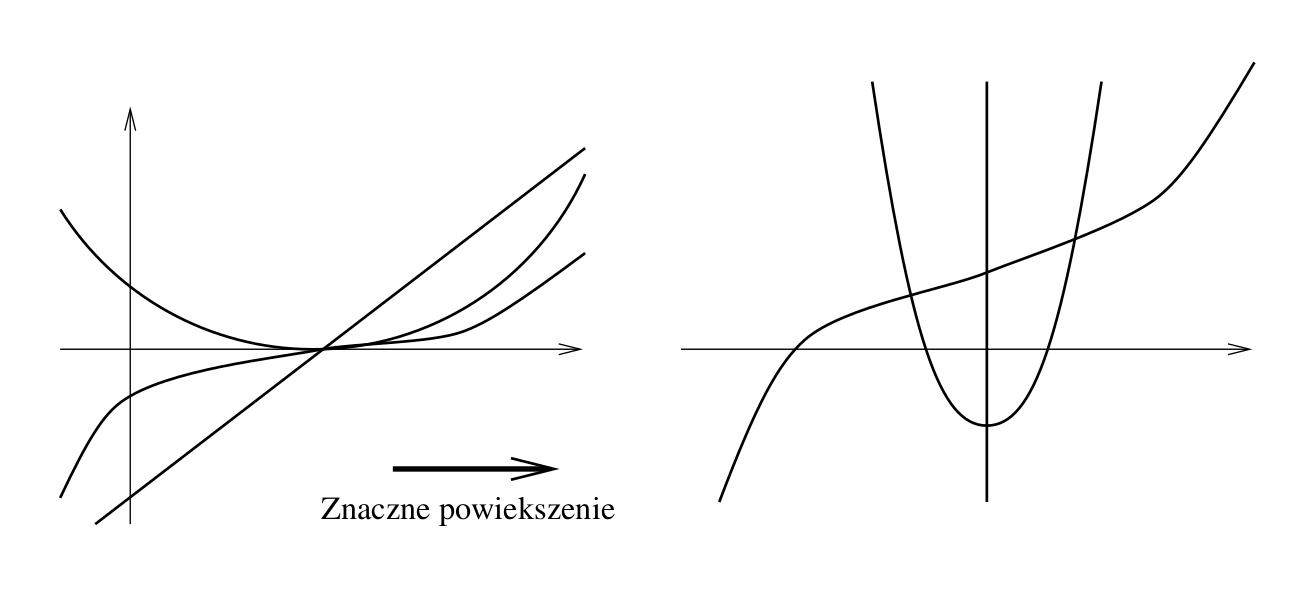
\includegraphics[width=\textwidth]{img/8/wielomian}
  \end{frame}

  \section{Deflacja -- dzielenie syntetyczne}

  \begin{frame}
    \textbf{Deflacja} -- bardzo użyteczny element wyznaczania pierwiastków wielomianów. % ELEMENT???

    \textit{Nested form (Horner)}:

    $$ f(x) = \sum_{i=0}^m a_i \cdot x^i = ( ( \dots (( a_m \cdot x + a_{m-1}) \cdot x + a_{m-2} ) \cdot \dots) \cdot x + a_1) \cdot x + a_0 $$
  \end{frame}

  \begin{frame}
    Rekurencyjny algorytm obliczania wartości wielomianu dla $x = \lambda$ ma postać:

  $$ \left \{ \begin{array}{l}
  b_{m-1} = a_m \\
  b_i = a_{i+1} + \lambda \cdot b_{i+1}, \quad i = m - 2, m-3, \dots, 0 \\
  f( \lambda ) = a_{0} + \lambda \cdot b_{0}
  \end{array} \right. $$
  \end{frame}

\end{document}
